% article draft

\documentclass[oneside,12pt]{article}
\usepackage[a5paper,margin=5mm]{geometry}%,showframe
%\usepackage{showframe}
\usepackage[utf8]{inputenc}
\usepackage{hyperref}
\usepackage[pdftex]{graphicx}

\newcommand{\email}[1]{$<$\href{#1}{#1}$>$}

\title{Using active hypergraph database\\as software development approach:\\\Huge{Graph Driven Programming}}
\author{\small{\copyright\ Dmitry Ponyatov \email{dponyatov@gmail.com}, free researcher, 2017}}

\begin{document}
\maketitle
%\tableofcontents

\begin{abstract}\noindent
Software development and program architecture engineering has grows complexity in last decades. The existing zoo of programming languages, para\-digms, hardware platforms and operating systems, combined with the software development market requirements, exceeds the capabilities of a particular individual developer. Thus, it is required to create a powerful tool for compensation of software systems development complexity, that combines design tools, RAD, MDP, simulation debugging, static and dynamic analysis of programs, parallel computing support, and, first of all, an expert system and knowledge bases provides knowledge storage, fuzzy search and inference not only in software engineering, but also in applied fields (mathematics and numerical methods, physics, chemistry, mechanics and structural engineering, CAD, electronics, digital signal processing, business planning, accounting and logistics, task and time management, etc).
\end{abstract}

\noindent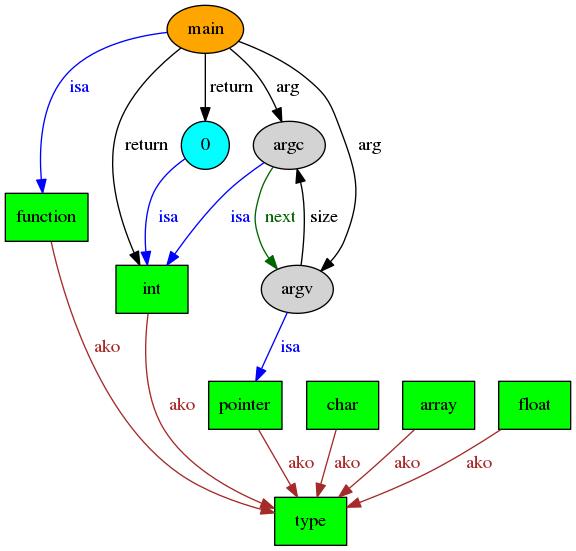
\includegraphics[width=\textwidth]{fig/hello.png}

\noindent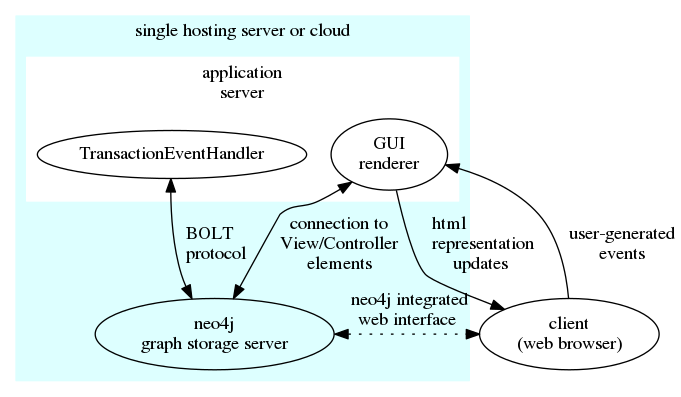
\includegraphics[width=\textwidth]{fig/architecture.png}

\noindent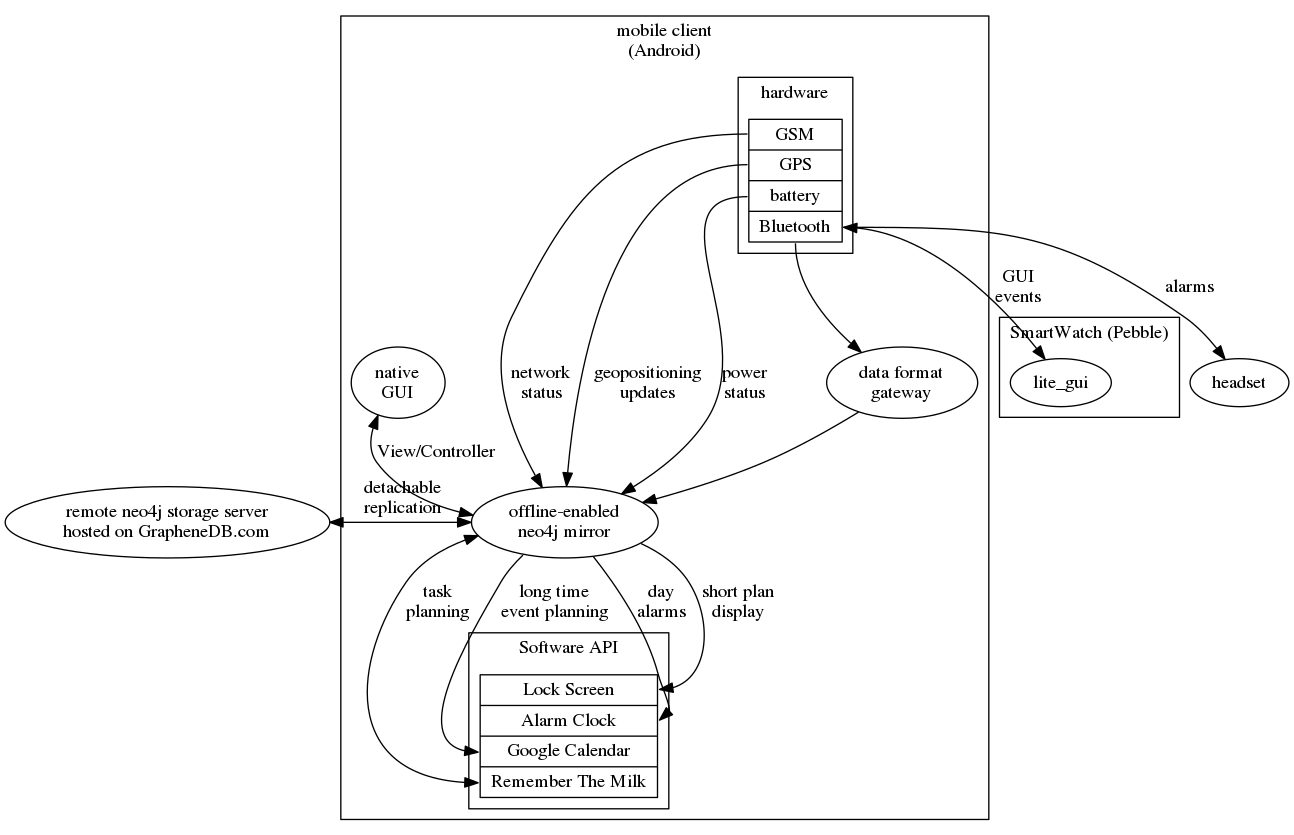
\includegraphics[width=\textwidth]{fig/mobile.png}

\noindent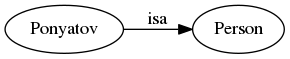
\includegraphics[width=0.5\textwidth]{fig/person.png}

\end{document}
